\SetTitle{31}{The Quantum Fourier Transform}{Phase estimation in reverse}{31}

\begin{frame}{Overview}{What will we study?}

\begin{itemize}
    \item The \href{https://en.wikipedia.org/wiki/Fourier_transform}{Fourier Transform} is well known in physics and mathematics for its ability to represent a time-based signal as a summation of frequencies that approximates or yields the original signal.
    \item We will review the basics of the classical Fourier transform.
    \item We will study the Quantum Fourier Transform (QFT), but it turns out that this circuit is simply the \href{https://en.wikipedia.org/wiki/Quantum_phase_estimation_algorithm}{Phase Estimation} circuit, executed in reverse.
    \item The QFT is at the center of important quantum algorithms, such as \href{https://en.wikipedia.org/wiki/Shor\%27s_algorithm}{Shor's Algorithm}, which we study next.
\end{itemize}
\end{frame}

\section*{Classic Fourier}

\begin{frame}{Classic Fourier}{Overview}
\Vskip{-3em}\TwoColumns{%
\Vskip{-2.5em}\begin{center}
        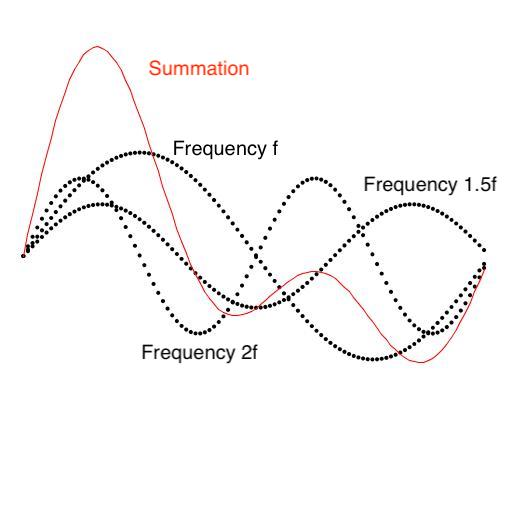
\includegraphics[width=0.8\textwidth]{31/instr.jpeg}
    \end{center}
}{%
\begin{itemize}
    \item Sine waves are plotted above at frequencies $f$, $2f$, and $1.5f$.
    \item If those frequencies sound at the same time, the red wave shows the resulting signal that reaches our ears:  the summation of the three black waves.
\end{itemize}
}
\Vskip{-1.5em}\begin{itemize}
    \item Remarkably, our brain performs Fourier analysis on the red signal, informing us that we hear a pitch, an octave above that pitch, and the ``fifth'' in between the other two pitches.
    \item This is how our brain can distinguish the sound of a slide trombone from a pipe organ.
   
\end{itemize}

\end{frame}